%%%%%%%%%%%%%%%%%%%%%%%%%%%%%%%%%%%%%%%%%%%%
\section{Risultati con parametri predefiniti}\label{ch:default}
Come già anticipato nella \autoref{ch:pythia_deuteron}, un parametro importante nella produzione deuteronica è \ttbox{norm}, che nel caso predefinito assume il valore di 119.6.
Tuttavia questo valore è stato ottenuto considerando l'energia iniziale del centro di massa a $\sqrt{s} = 7$ TeV, a differenza del valore di $\sqrt s = 13$ TeV considerato in questa tesi.
Perciò è lecito aspettarsi, a partire da questa considerazione, che vi sia una discrepanza nella produzione di (anti)deuteroni tra le simulazioni e i dati reali.
Per confrontare i dati delle simulazioni con i dati sperimentali si sono considerate le misure effettuate da ALICE riguardanti collisioni $pp$ a rapidità centrali ($|y|<0.5$) con energia del centro di massa $\sqrt s = 13$ TeV.
I dati dei protoni e dei (anti)deuteroni utilizzati in questa tesi sono tratti rispettivamente da \cite{ALICE:2020jsh} e da \cite{ALICE:2020foi}.\\

\begin{figure}[htb]
    \centering
    \begin{subfigure}{.49\textwidth}
    \centering
        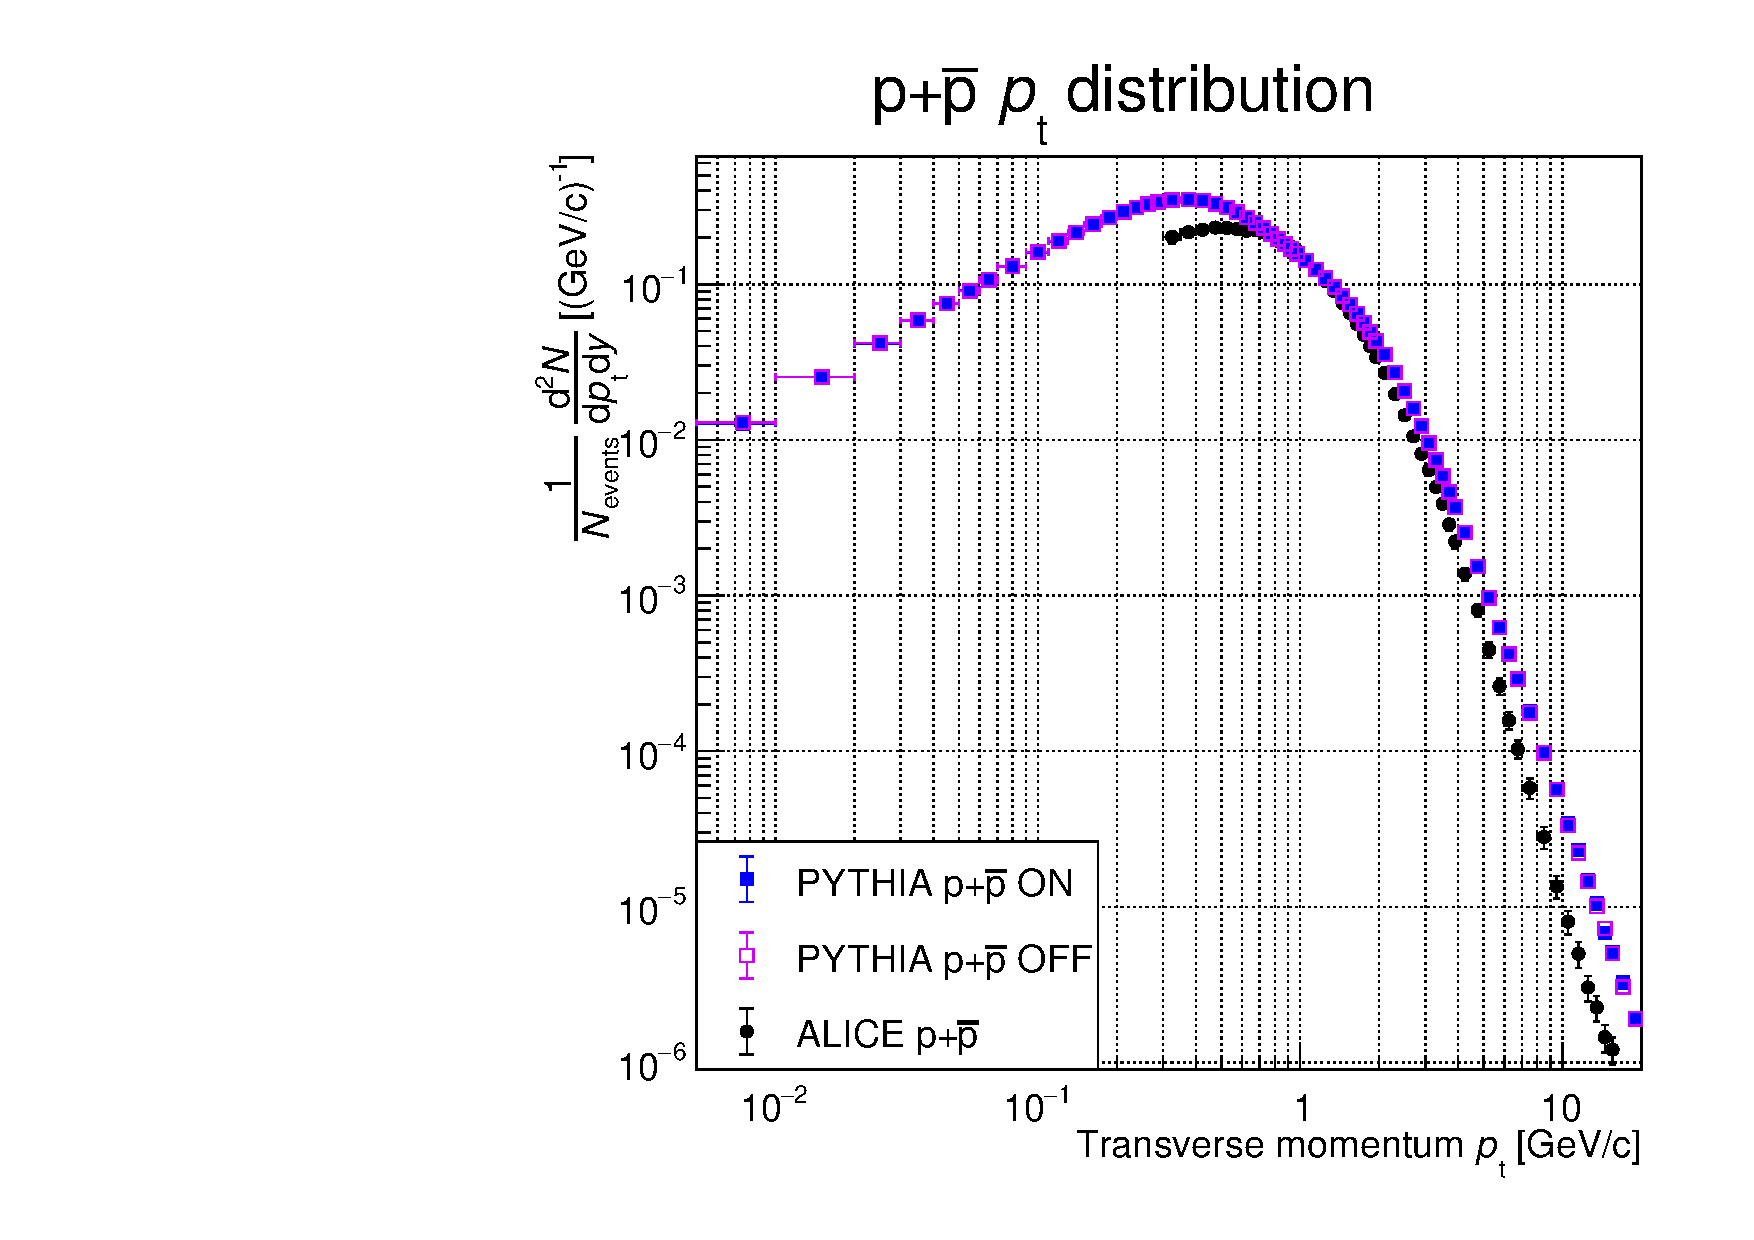
\includegraphics[width=\textwidth]{image/3-risultati/analyse/A/pp.pdf}
        \caption{}
        \label{fig:A_pp}
    \end{subfigure}
    %\hspace{1cm}
    \begin{subfigure}{.49\textwidth}
        \centering
        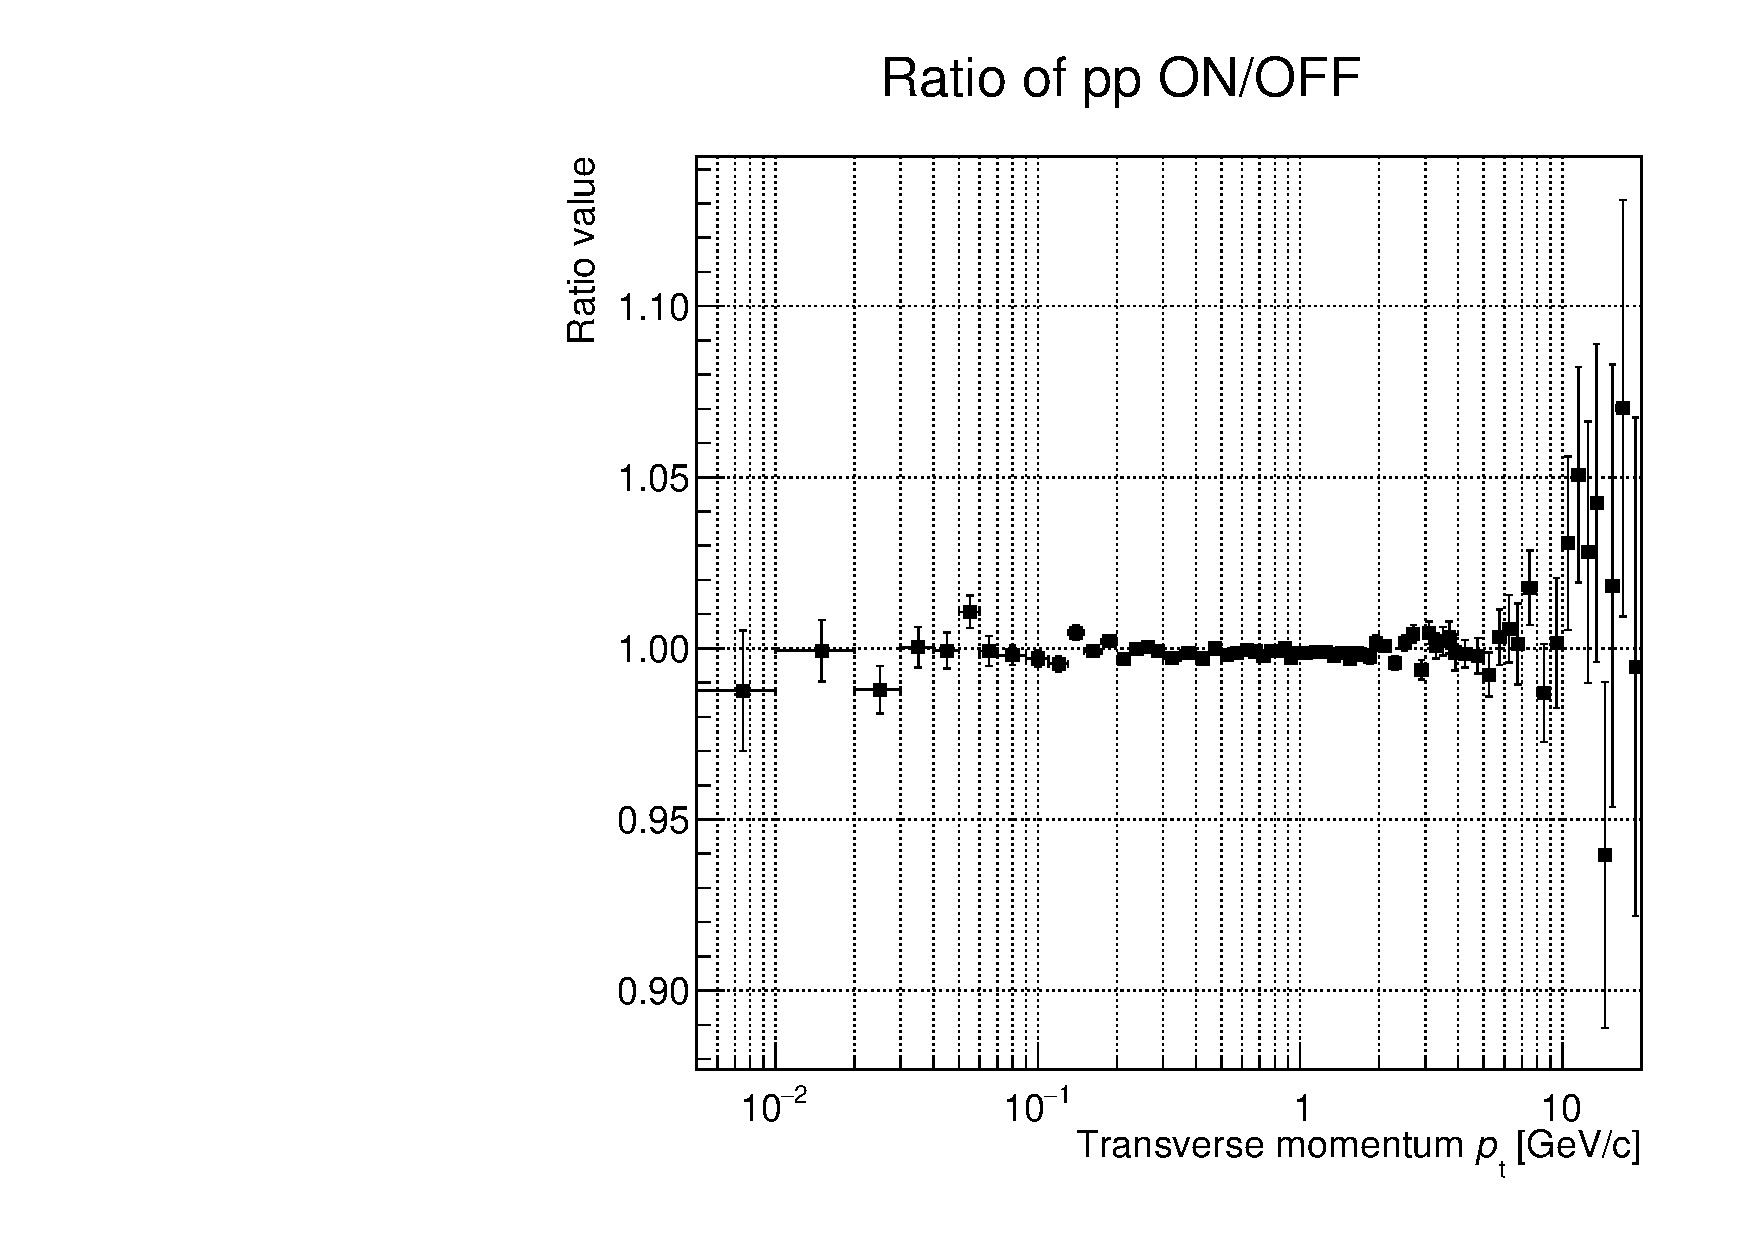
\includegraphics[width=\textwidth]{image/3-risultati/analyse/A/ratio_pp_ON_OFF.pdf}
        \caption{}
        \label{fig:A_ratio_pp_ON_OFF}
    \end{subfigure}
    \captionwithsource{\emph{\rmfamily (a)} Distribuzione dell'impulso trasverso di $p+\bar p$ con produzione deuteronica attivata e disattivata ("ON" e "OFF") in confronto con i dati sperimentali di ALICE ("ALICE"). \emph{\rmfamily (b)} Frazione della distribuzione dell'impulso trasverso di $p+\bar p$ con produzione deuteronica attivata e con produzione non attivata.}{\cite{ALICE:2020jsh}}
    \label{fig:A_pp_prod}
\end{figure}
Eseguendo la simulazione una volta con i parametri predefiniti e una volta con la produzione deuteronica disattivata (\ttbox{HadronLevel:DeuteronProduction = off}), otteniamo i vari spettri di produzione.
Ci si aspetta una piccola differenza tra il caso in cui la produzione di deuteroni è attivata e non, in particolare il numero di protoni dovrebbe essere leggermente minore in cui la produzione si attivata, visto che una parte di questi si ricombina per formare un deuterone.
Dalla \autoref{ch:objectives_alice} sappiamo che il numero di deuteroni prodotti deve essere circa 1000 volte inferiore al numero di protoni, per cui il rapporto tra numero di protoni con produzione (anti)deuteronica attivata e disattivata dovrebbe avvicinarsi al valore di 0.999.
\begin{figure}[htb]
    \centering
    \begin{subfigure}{.49\textwidth}
    \centering
        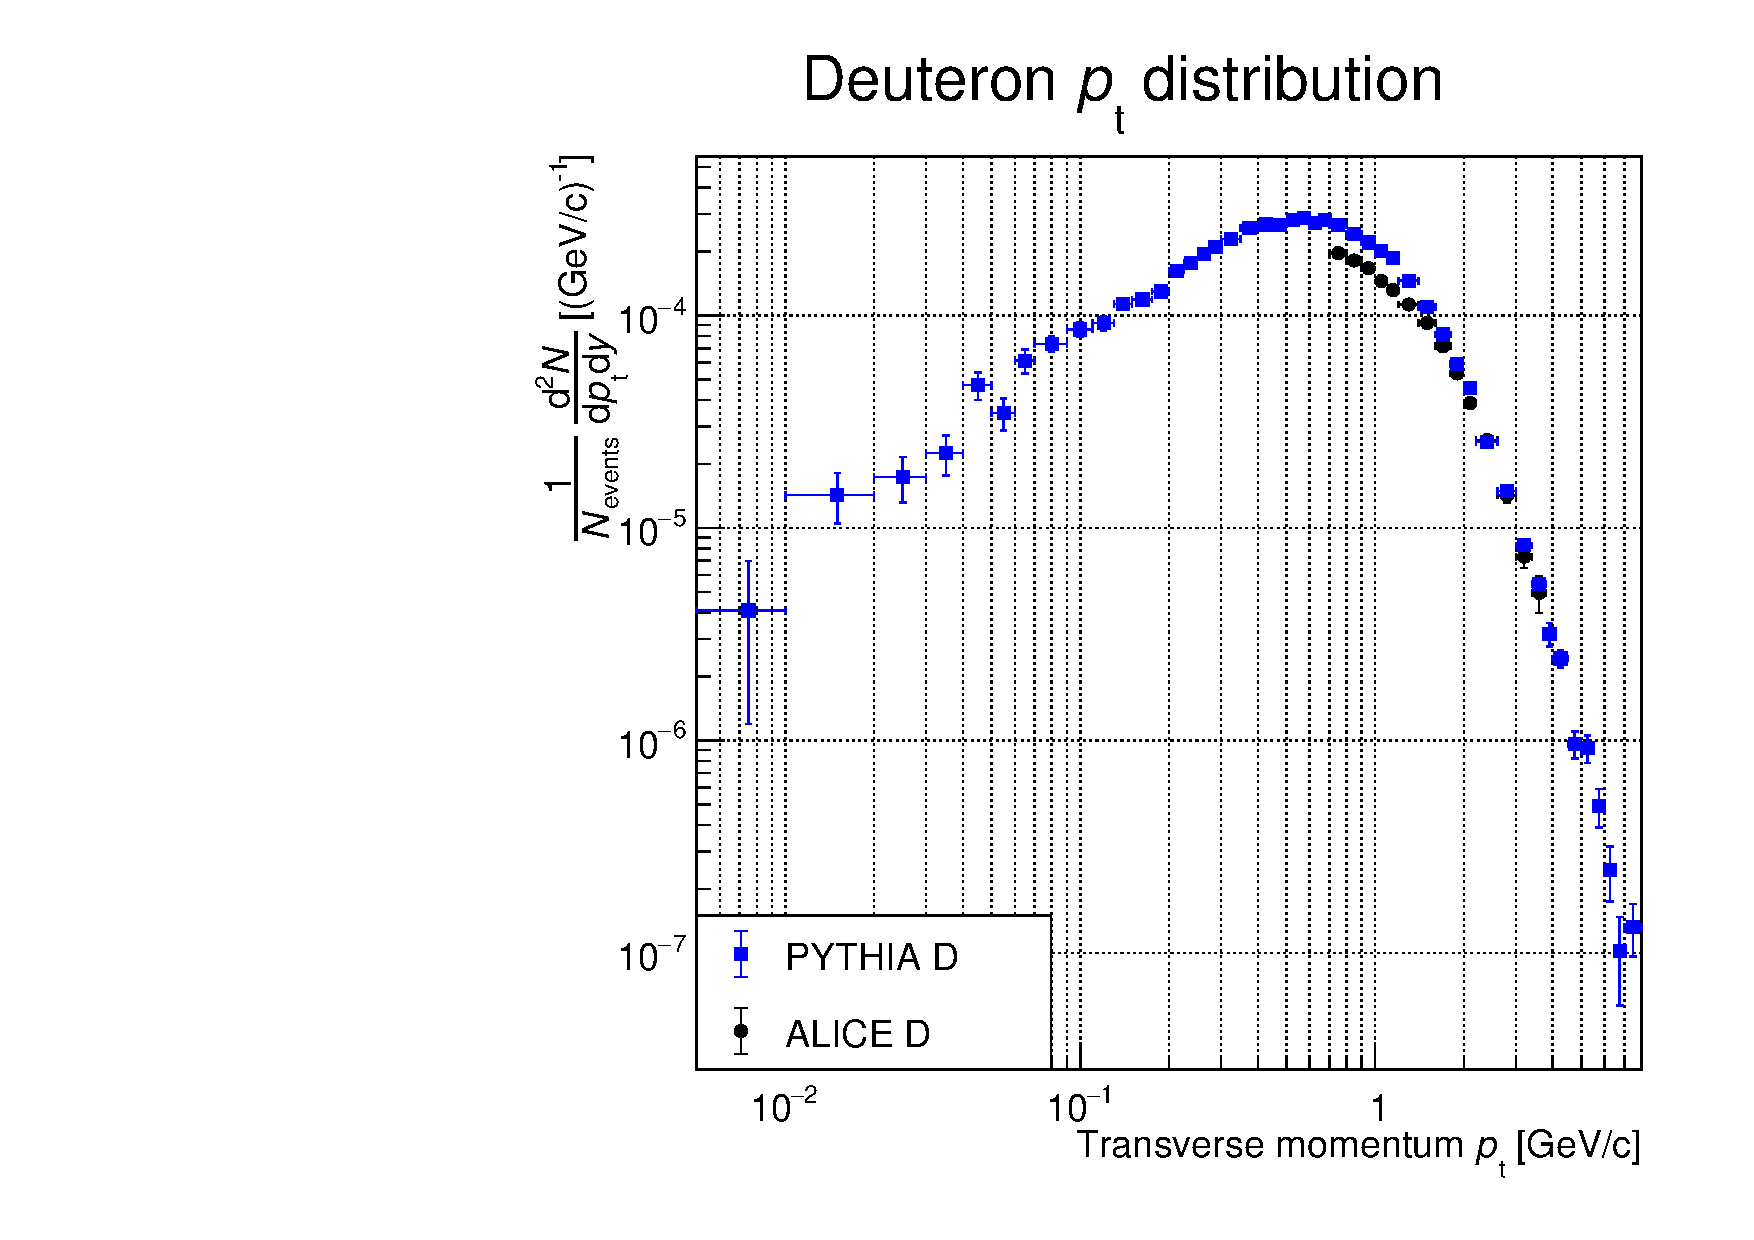
\includegraphics[width=\textwidth]{image/3-risultati/analyse/A/deuteron.pdf}
        \caption{}
        \label{fig:A_deuteron}
    \end{subfigure}
    %\hspace{1cm}
    \begin{subfigure}{.49\textwidth}
        \centering
        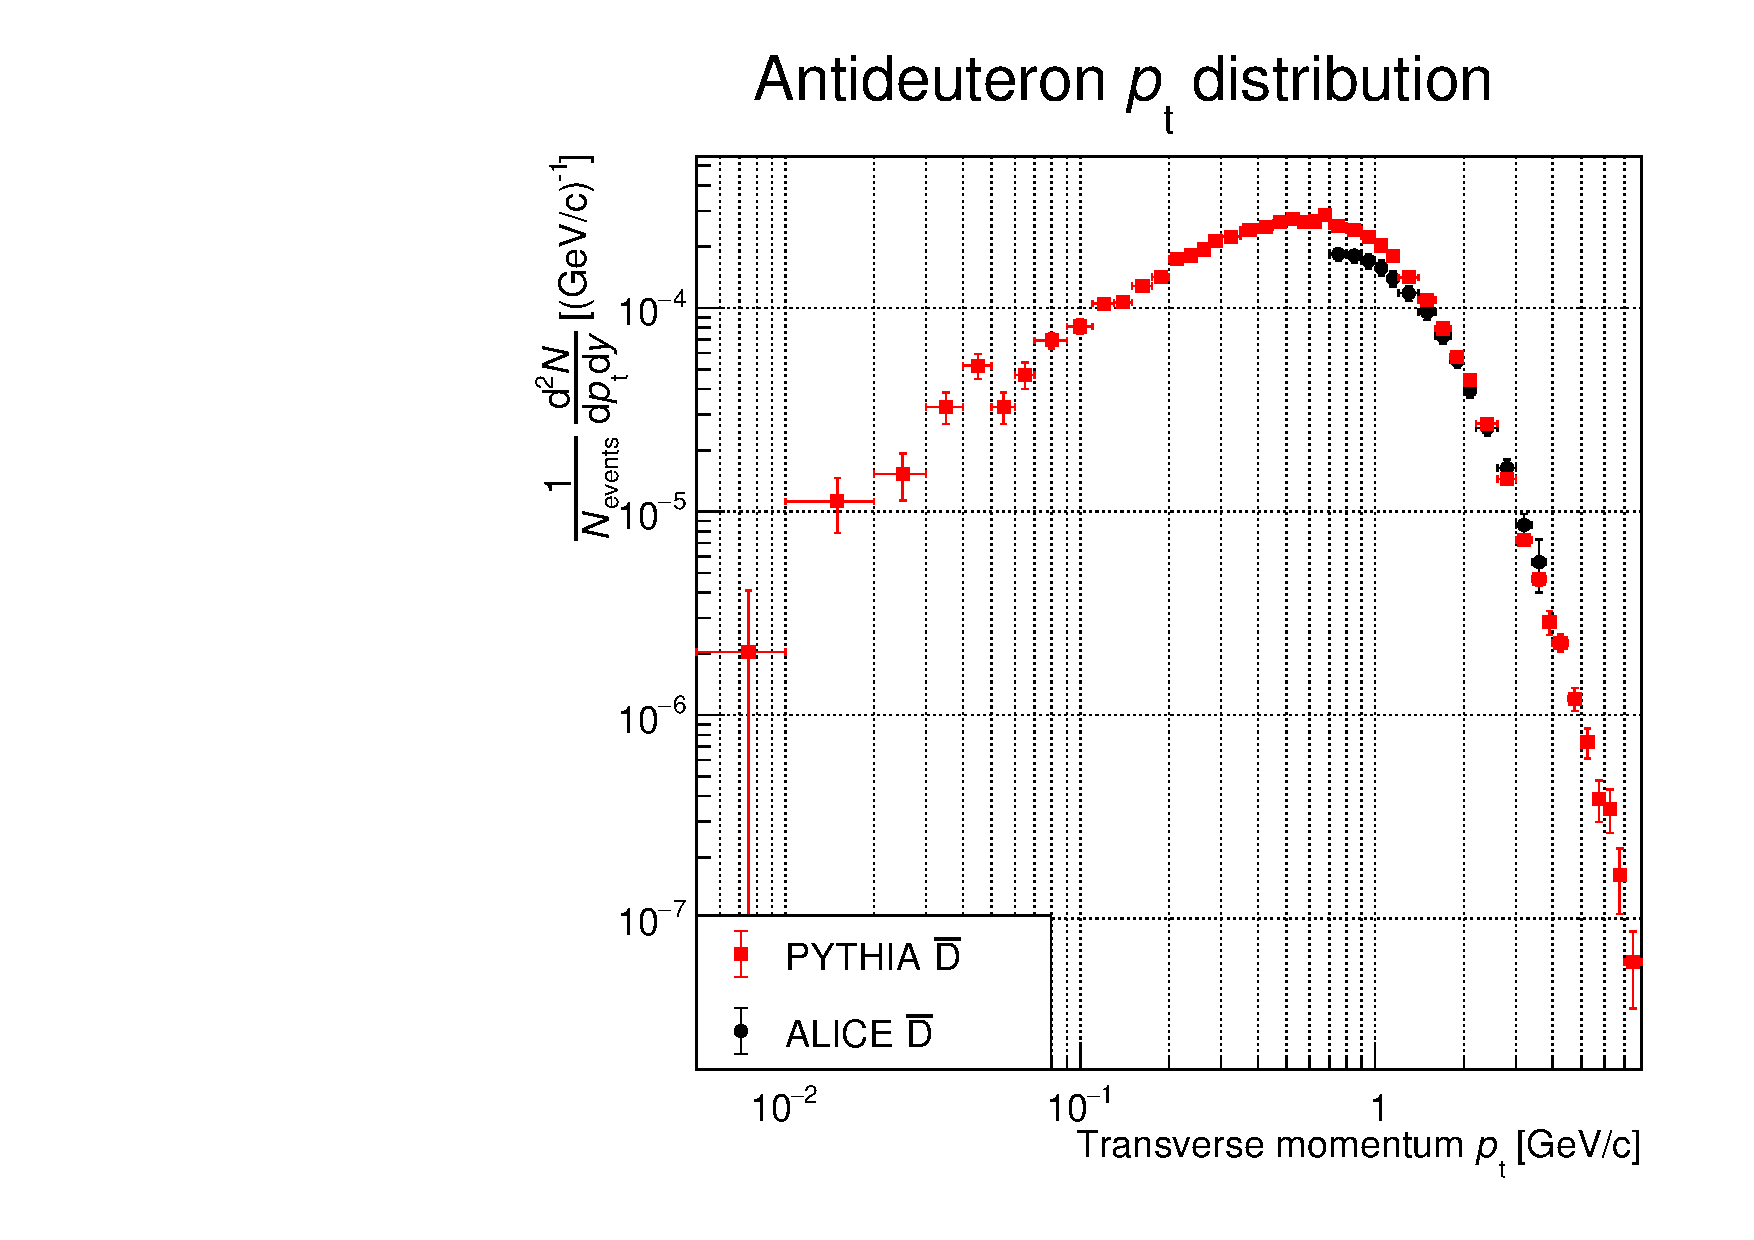
\includegraphics[width=\textwidth]{image/3-risultati/analyse/A/antideuteron.pdf}
        \caption{}
        \label{fig:A_antideuteron}
    \end{subfigure}
    \captionwithsource{Distribuzione dell'impulso trasverso di \emph{\rmfamily (a)} $D$ e \emph{\rmfamily (b)} di $\bar D$ in confronto con i dati di ALICE.}{\cite{ALICE:2020foi}}
    \label{fig:A_(anti)deuteron}
\end{figure}

In \autoref{fig:A_pp} osserviamo lo spettro di produzione della somma di protoni e antiprotoni nel caso in cui la produzione deuteronica sia attivata e non attivata, messo in confronto con i dati sperimentali.
Da questo grafico possiamo dedurre che la riproduzione di \pythiaa{} dello spettro dei protoni è fedele solamente nell'intorno di $p_t \sim 1$ GeV/$c$.
Gli andamenti degli spettri con produzione attivata e disattivata non presentano  particolari differenze, se non negli impulsi più alti, ma ciò è dovuto alle maggiori fluttuazioni dovute alla minore statistica.
Eseguendo un rapporto dei due istogrammi, visibile in \autoref{fig:A_ratio_pp_ON_OFF}, si ottiene che la media pesata del valore della frazione risulta essere $0.9988 \pm 0.0002$, inferiore a 1, compatibile con il valore atteso di 0.999.
Bisogna menzionare che le predizioni per la produzione di protoni da \pythiaa{} sono note per non descrivere fedelmente le misure sperimentali.
Questo è perché il tune di \pythiaa{} non è stato ottimizzato per riprodurre la produzione di nucleoni all'LHC, ma è comunque utilizzato come base per la maggior parte delle predizioni ed è stato utilizzato per la stima dei parametri per la sezione d'urto efficace, giustificando la scelta del \textit{tuning} per questo studio.
La produzione dei (anti)nuclei dipende essa stessa dallo spettro di produzione di protoni, che risulta interconnessa con tali parametri, ma la descrizione delle misure di protoni esula dallo scopo di questa tesi.

Se andiamo a confrontare invece lo spettro dei deuteroni e degli antideuteroni con i dati di ALICE \cite{ALICE:2020foi}, osserviamo in \autoref{fig:A_(anti)deuteron} che la produzione (anti)deuteronica è accurata solamente per gli impulsi più alti, nell'intorno di $p_t \sim 3$ GeV/$c$.
Infatti, eseguendo una divisione tra i dati di \pythia e di ALICE per i (anti)deuteroni, è possibile osservare che il rapporto si avvicina al valore unitario in quell'intorno, come si vede in \autoref{fig:A_division}.
In generale si osserva una sovrapproduzione sia per i deuteroni e sia per gli antideuteroni, con le medie pesate rispettivamente di $1.203 \pm 0.017$ e di $1.129 \pm 0.023$.
\begin{figure}[htb]
    \centering
    \begin{subfigure}{.49\textwidth}
    \centering
        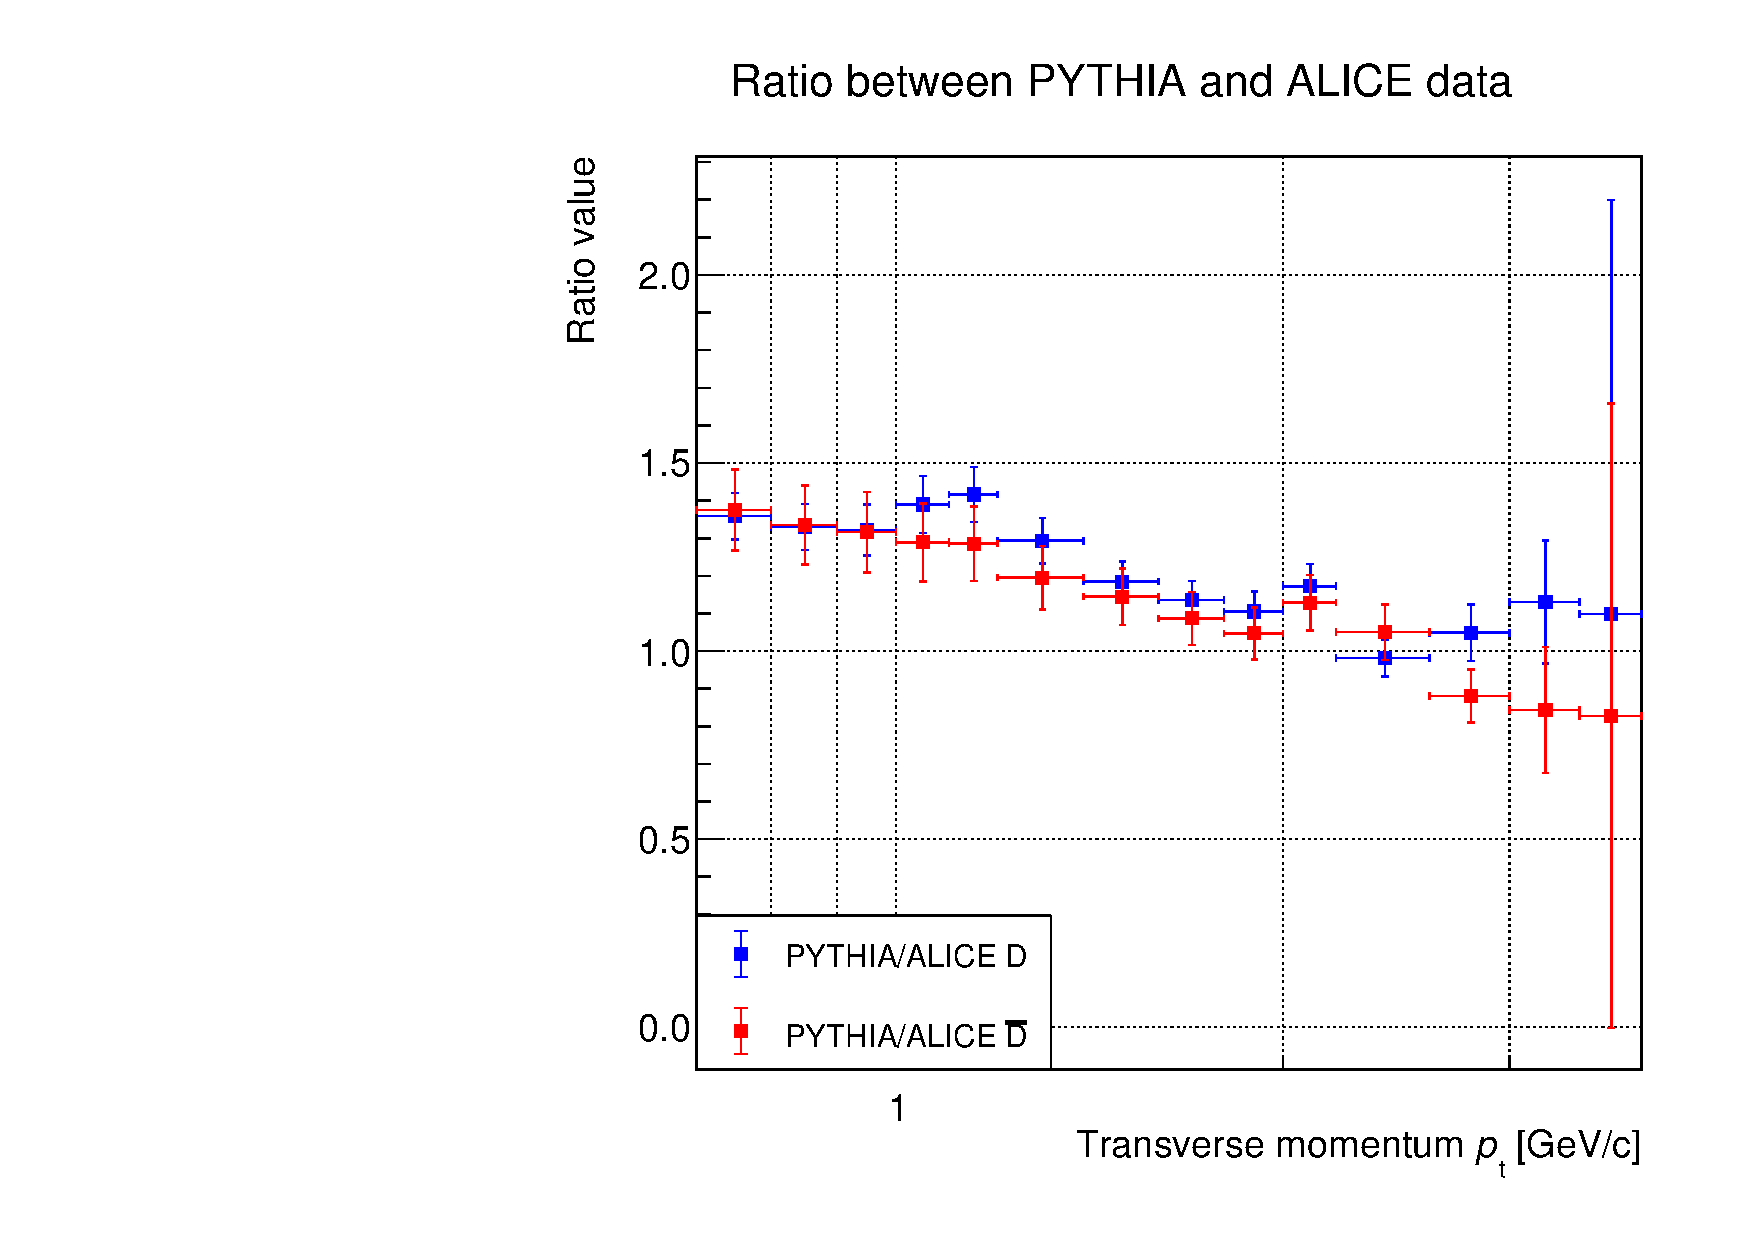
\includegraphics[width=\textwidth]{image/3-risultati/analyse/A/division.pdf}
        \caption{}
        \label{fig:A_division}
    \end{subfigure}
    %\hspace{1cm}
    \begin{subfigure}{.49\textwidth}
        \centering
        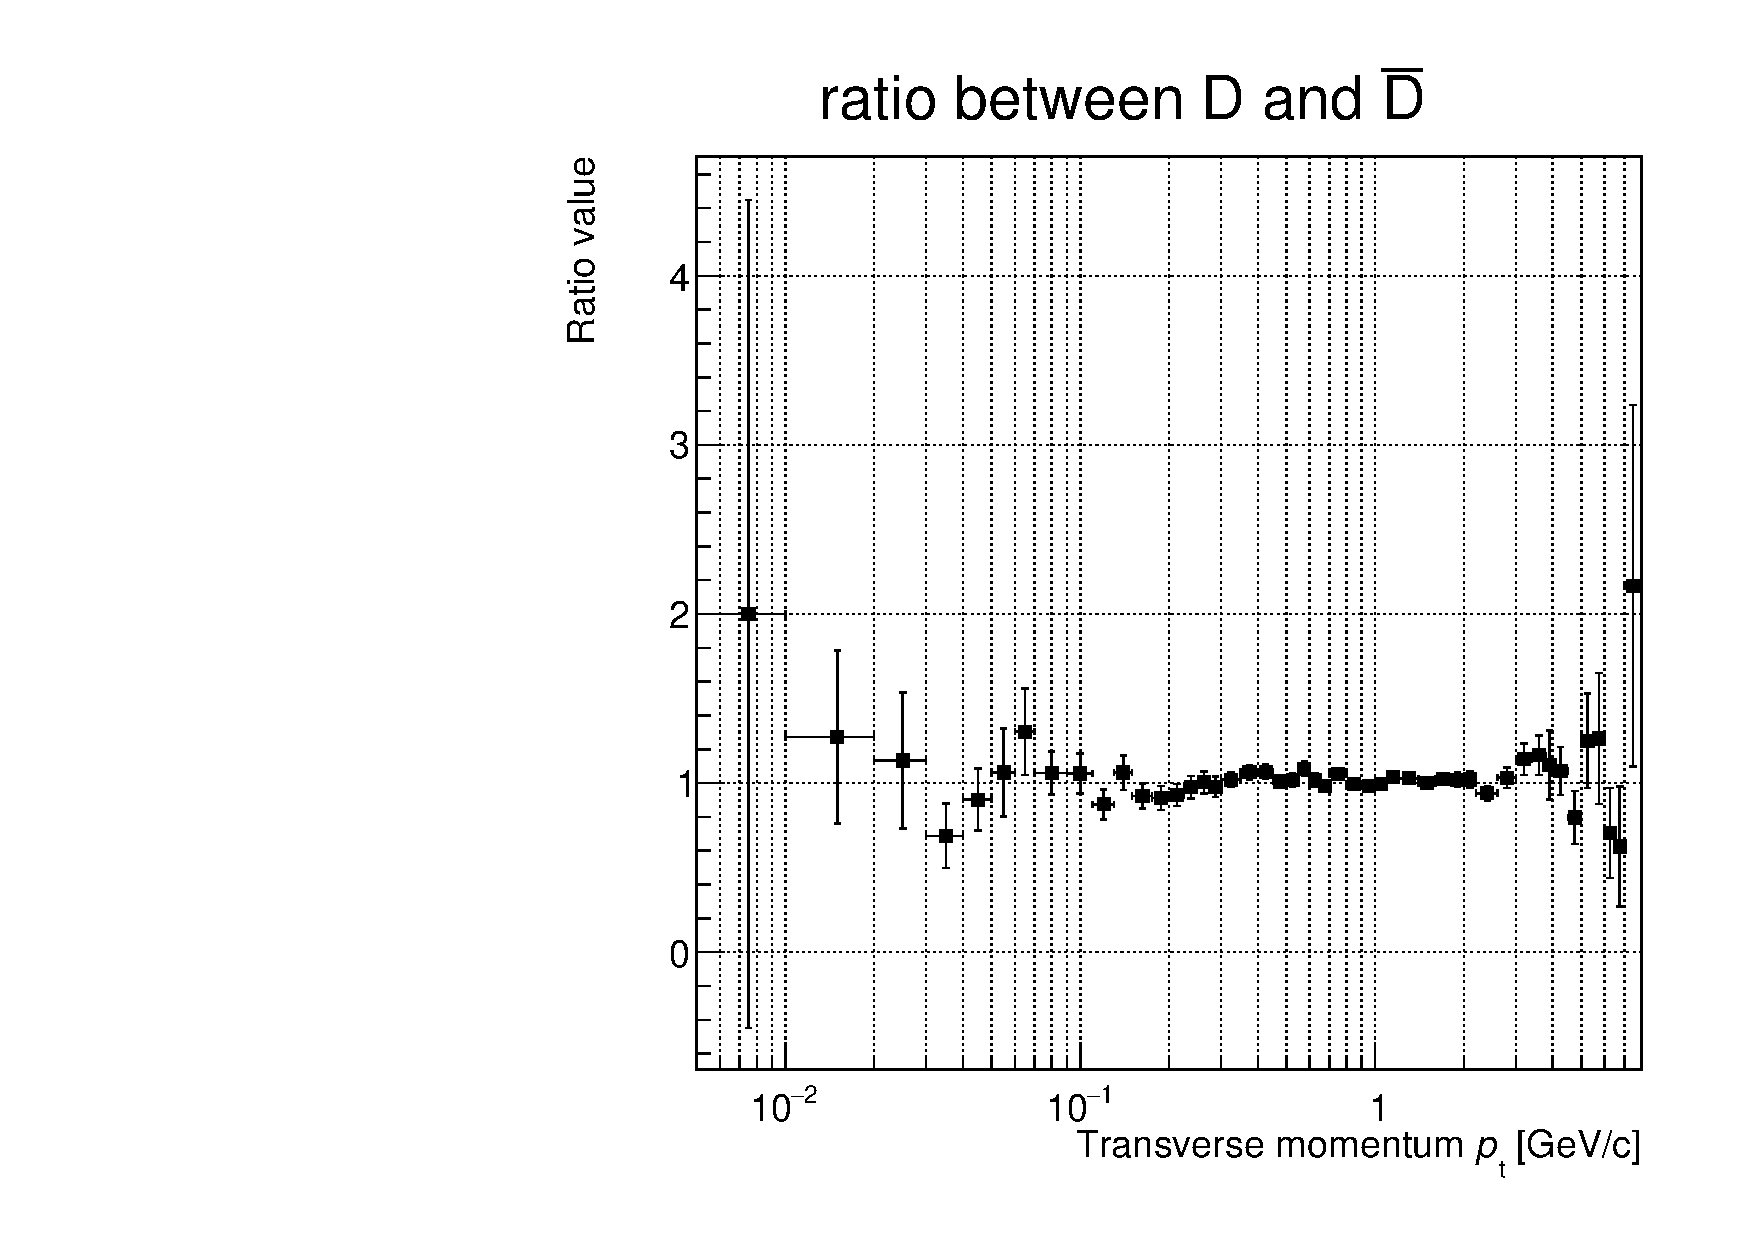
\includegraphics[width=\textwidth]{image/3-risultati/analyse/A/ratio_DD.pdf}
        \caption{}
        \label{fig:A_ratio_DD}
    \end{subfigure}
    \caption{\emph{\rmfamily (a)} Divisione tra la distribuzione dell'impulso trasverso di $D$ e $\bar D$ con i dati di ALICE. \emph{\rmfamily (b)} Rapporto delle distribuzione dell'impulso trasverso di $D$ con quello di $\bar D$.}
    \label{fig:A_ratio_DD_}
\end{figure}

Per verificare ulteriormente la correttezza delle predizioni si è fatto un ulteriore rapporto, riportato in \autoref{fig:A_ratio_DD}, tra lo spettro dei deuteroni e lo spettro degli antideuteroni.
La media pesata del rapporto risulta essere $1.013 \pm 0.008$, con una leggera sovrapproduzione di deuteroni.